%\documentclass{article}
\documentclass[a4paper,12pt]{article}
% Seitenränder in schön für Steven
\usepackage[paper=a4paper,left=25mm,right=25mm,top=25mm,bottom=25mm]{geometry}
\usepackage{enumitem}
\usepackage{amsmath}
\usepackage{graphicx}
\usepackage{tikz}
\usepackage{titling}


% Schusterjungen und Hurenkinder bestrafen
\clubpenalty50000
\widowpenalty50000
\displaywidowpenalty=50000

% Buchstaben mit kringel drum: %
\newcommand*\mycirc[1]{%
	\begin{tikzpicture}[baseline=(C.base)]
	\node[draw,circle,inner sep=1pt](C) {#1};
	\end{tikzpicture}}

\author{Benedict Hans, Christoph Dollase, Steven Te\ss endorf}
\setlength{\droptitle}{-5em} % set the title to the top of the page

% ==========================
% ===== START HERE!! =======
% ==========================
\title{ \textbf{Problem Sheet 6}}
\setcounter{section}{6} % Nummer des Aufgabenblattes

\begin{document}	 
	\maketitle	 %Some Vodoo-magic
	
	\subsection{Modulation 2}
	\textbf{Consider the following modulation diagram.}
    
	\begin{figure}[h!]
		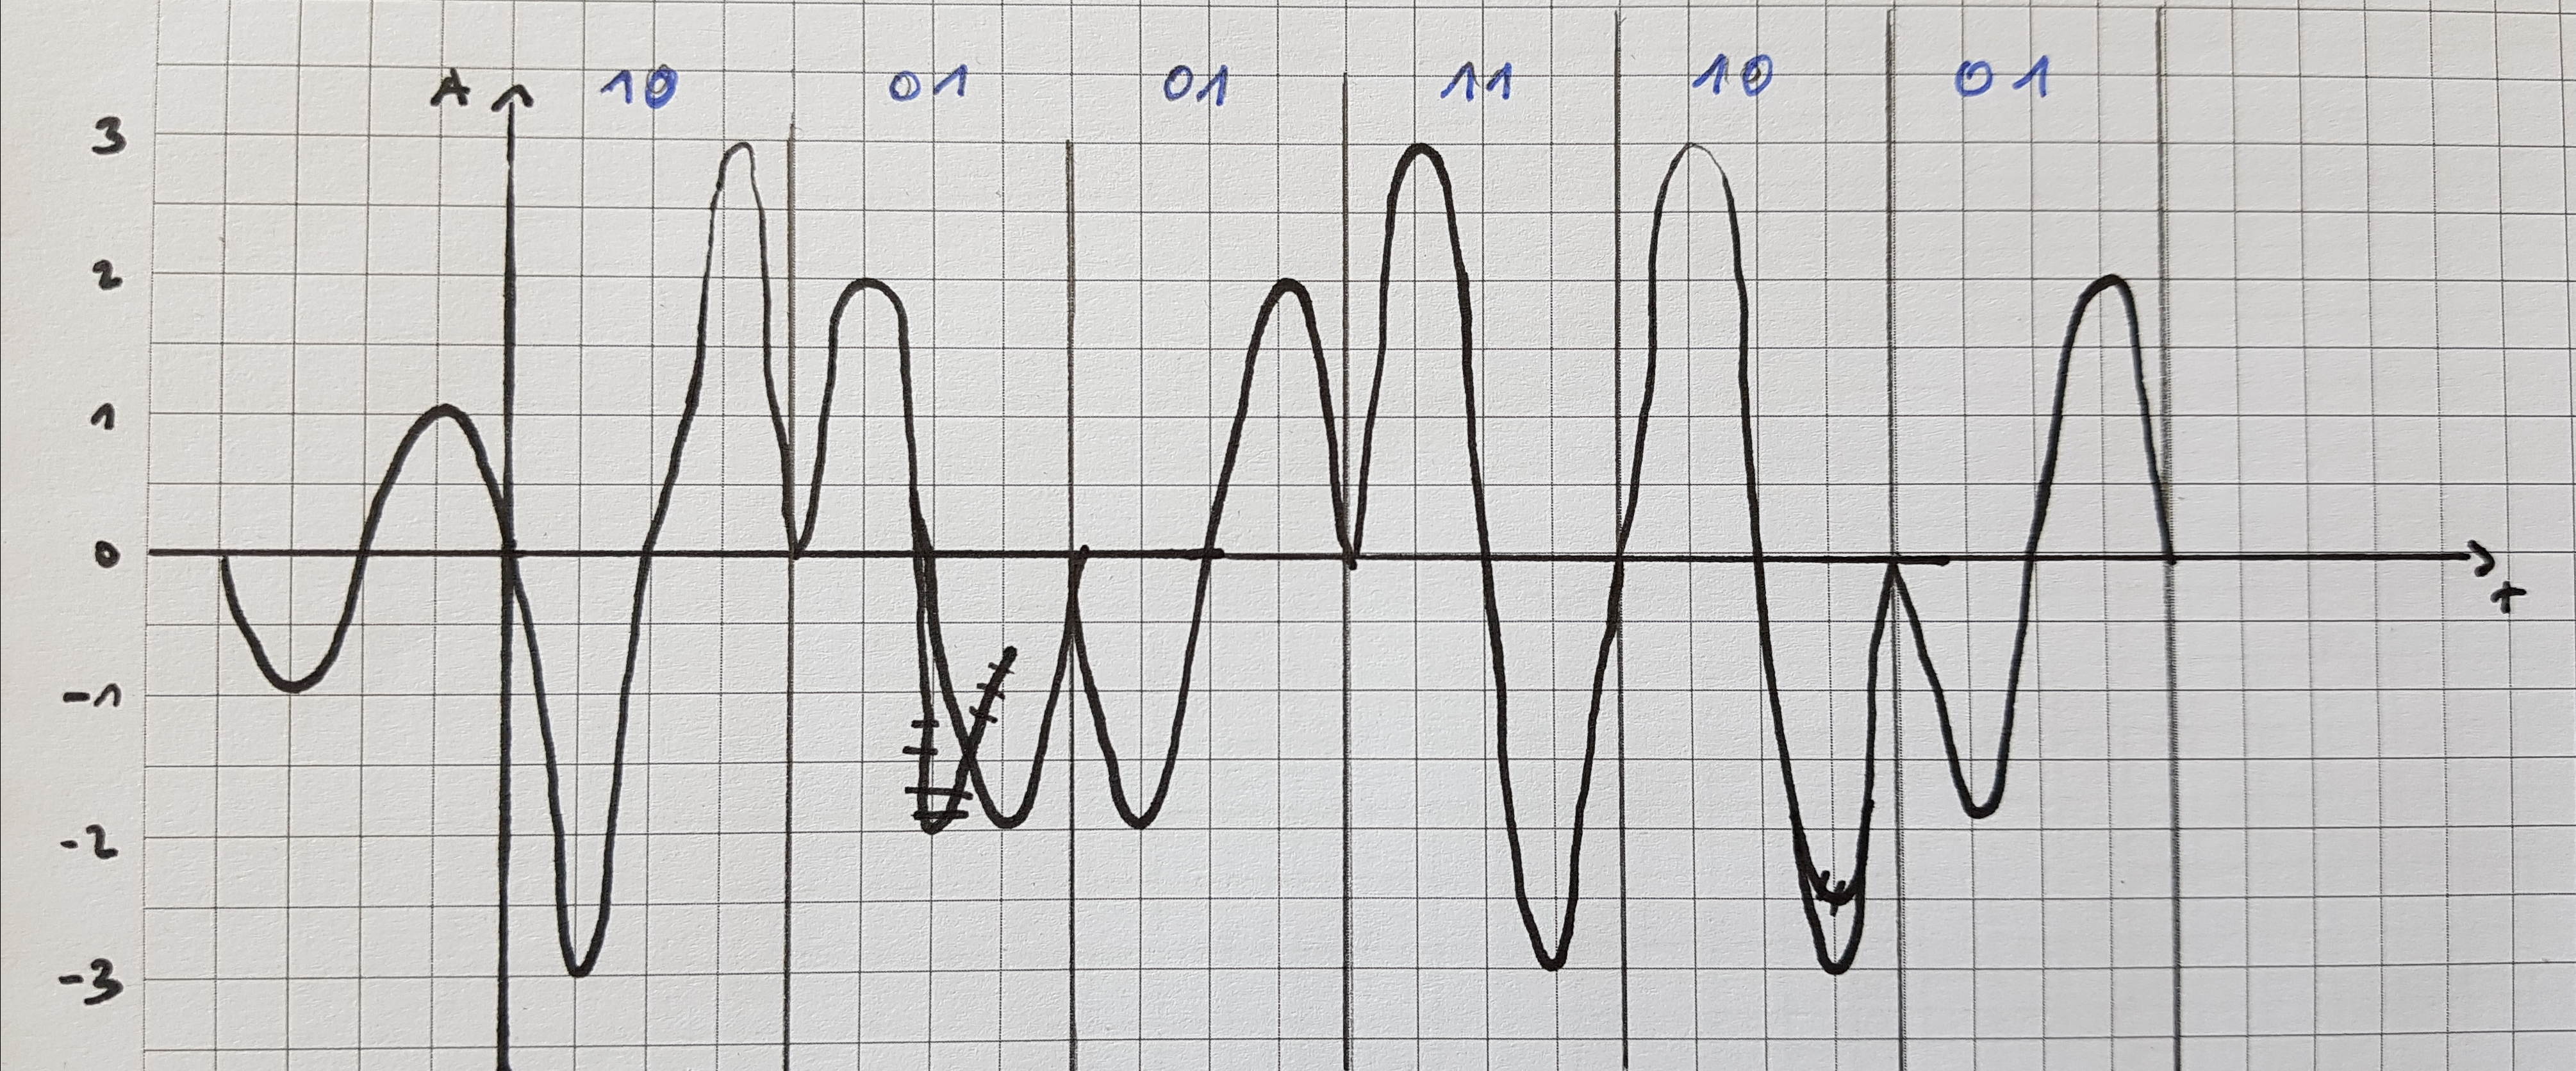
\includegraphics[width=0.4\linewidth]{modulation.png} 
    	\caption{Modulationgraph}
	\end{figure}
    
    \textbf{The signal has already been sampled and demodulated. The symbols are depicted in the 
	modulation diagram. Specify the (de-)modulation table for the applied (de-)modulation scheme.
	Sketch the corresponding constellation diagram.}

    \begin{figure}[h!] 
        \includegraphics[width=1\linewidth]{mod_solution.png} 
	    \caption{Table and constellation diagram}
    \end{figure}
	
	\newpage
	
	\subsection{Modulation 3}
	\textbf{Modulate the bit sequence 100101111001 using a combination of amplitude and frequency
	shift keying. Each symbol shall be modulated for 1/2 T time units on the sine carrier wave.
	Use the information table in the assignment sheet.}
	
    \begin{figure}[h!] 
        \includegraphics[width=1\linewidth]{mod_solution2.png} 
	    \caption{Modultiongraph}
    \end{figure}
	
	% Solution
	
	\subsection{Last Mile Problem}
	\textbf{Explain the Last Mile Problem. What technologies are currently used on the last mile?}\\
\\	
	The most main hubs of the internet are connected among each other with very fast Gigabit connections. The bottleneck of the users speed is the so called last mile. That means the connection from the last switch station to the home of the user. In most cases the responsibility lies with local providers. Laying new cables is really expensive. Therefore the providers try to reuse existing connections, like old telephone lines. To provide acces to the internet different techniques were developed.
	
	\begin{itemize}
		\item Classical Modem (\textit{\textbf{Mo}dulator - \textbf{Dem}odulator})
		\begin{itemize}
			\item AC (Alternating Current) signaling is used
			\item Sine wave carrier is used (famous modem sound)
			\item Amplitude, frequency, or phase is modulated to transmit data
		\end{itemize}
		\item Integrated Services Digital Network (ISDN)
		\begin{itemize}
			\item Integration of different communication services (voice, fax, data, ...)
			\item Digital communication
			\item Higher capacity than modem-based data transfer
			\item Uses existing infrastructure: ISDN is no new network, but something added to an existing network
		\end{itemize}
		\item Digital Subsriber Line (DSL)
		\begin{itemize}
			\item Combination of usual phone service (analog/ISDN) and data service
			\item uses the whole frequency spectrum of copper cable (ISDN: <3.4kHz)
			\item Data rate depends on distance to the switching center and the cable quality
			\item Discrete Multitone Modulation (DMT) or Carrierless Amplitude Phase Modulation (CAP)
		\end{itemize}
	\end{itemize}
	
	\subsection{Transmission Time}
	\textbf{\textit{See stock market example in assignment sheet!}}
	\begin{enumerate}[label=(\roman*),itemsep=0pt]
		\item \textbf{How far are these cities away?  How long would it take a wireless signal at the speed of light
			to travel this distance?}
		\begin{itemize}
			\item distance between Berlin and New York: $6.381 ~km$
			\item speed of light $c$ = $299.792.458 ~m/s$: $s = v \cdot t$ $\rightarrow$ $t = s / v $ \\
			$t = \frac{6.381.000}{299.792.458} = 0,0213 ~s$ = $21,3 ~ms$
		\end{itemize}
		\item \textbf{A signal in the electromagnetic short wave band may have the physical properties to travel this distance within this time.  However, channel bandwidth and thus baud rate are very much limited.  Assume you were granted access to a 20 kHz channel in this band. Expect a signal-to-noise ratio of -13.5 dB. What a bit rate could you achieve?}
		\begin{itemize}
			\item Shanon: noise ratio of -13.5 $dB$ $\rightarrow$ $SNR = 0.04467$ (noise > signal)\\
			$data~rate = 20.000 \cdot log_2( 1+ 0.04467) = 1,26 ~bit/s$
		\end{itemize}
		\item \textbf{Let us try encoding a message for the application. For buying stocks (identified by a 4-digit name), we only need a short message format, for example:  {\large BUY 2000 DJIA}\\
		How long does it take to transmit this message? Assume ASCII encoding and the bitrate you have calculated.}
		\begin{itemize}
			\item $[BUY~2000~DJIA]_{lit} = [66~85~89~\textcolor{blue}{32}~50~48~48~48~\textcolor{blue}{32}~68~74~73~65]_{ascii}$ (13 symbols)
			\item ASCII is encoded via 8 bit per symbol $\rightarrow$ $13 \cdot 8 = 104$ Bits to transport
			\item $t = \frac{104}{1,26} = 82.54~s$
		\end{itemize}
		\item \textbf{Would the short wave transmission be faster than the internet transmission?}
		\begin{itemize}
			\item the typical short wave transmission uses frequencies between  1.7-30 $MHz$  $\rightarrow$ it is 80-1500 times faster the given 20 $kHz$ channel.
		\end{itemize}
	\end{enumerate}
	
	
	
\end{document}

% Hier nach passiert nichts mehr, daher nutzen wir das als kleines Cheat-Sheet ;)
% ===============================================================================

% Aufzählungen (auch merhstufig):
\begin{itemize}[itemsep=0pt]
	\item 
\end{itemize}

%Bilder eifnügen:
\begin{figure}[h!] %h! sorgt dafür dass das Bild möglichst nicht woanders hingeschoben wird
	%Erklärung: [width=0.5\linewidth] -> Bild ist maximal so breit wie die Hälfte des Schriftbildes
	\includegraphics[width=0.5\linewidth]{Bildname.jpg} 
	\caption{Bildunterschrift}
\end{figure}

%Tabelle einfügen:
\begin{table}[h!] %h! sorgt dafür dass die Tabelle möglichst nicht woanders hingeschoben wird
	\caption{Tabellenüberschrift}
	%hinter {tabular}: Anzahl Spalten (c=center, l=linksbündig, r=rechtsbündig, | Spaltenstriche)
	\begin{tabular}{|c|c|c} 
		A & B & C  \\ % \\ = return (neue zeile)
		\hline % horinzontale Linie
		0 & 1 & 2
	\end{tabular}
\end{table}
